\documentclass[preprint,12pt]{elsarticle}

\usepackage{amsmath,amssymb,amsthm}
\usepackage{graphicx}
\usepackage{booktabs}
\usepackage[hidelinks]{hyperref}
\usepackage{xurl}
\usepackage{microtype}
\biboptions{numbers,sort&compress}

\newtheorem{theorem}{Theorem}
\newtheorem{lemma}{Lemma}
\newtheorem{proposition}{Proposition}
\newtheorem{corollary}{Corollary}
\theoremstyle{definition}
\newtheorem{definition}{Definition}

\newcommand{\Res}{R}
\newcommand{\per}{P}
% Generated by paper/analysis/analyze.py. Values are numbers (percent signs are added in the text).
\newcommand{\AccMape}{3.0}
\newcommand{\AccMapeBase}{3.0}
\newcommand{\AccMapeBaseAll}{3.0}
\newcommand{\AccMax}{18.7}
\newcommand{\AccMaxBase}{19.1}
\newcommand{\AccN}{118}
\newcommand{\AccNAll}{118}
\newcommand{\AccRankPct}{80}
\newcommand{\AccRankBasePct}{74}
\newcommand{\AccRankPairs}{66}
\newcommand{\HwBw}{12.3}
\newcommand{\MeasPenaltyMax}{1.50}
\newcommand{\MeasPenaltyMaxR}{21}
\newcommand{\MeasPenaltyMaxK}{2}
\newcommand{\MeasPenaltyMaxWorkload}{pre 256}


\journal{Preprint}

\begin{document}

\begin{frontmatter}

\title{Where Should Resident Layers Go? Optimal Placement for Weight Streaming in Offloaded LLM Inference}

\author[buv]{Quang-Vinh Dang\corref{cor1}}
\ead{vinh.dq4@buv.edu.vn}
\author[uef]{Dat Le}
\ead{datla@uef.edu.vn}
\author[mil]{Minh Ngoc Dinh}
\ead{minh.dinh@maeducation.com}
\cortext[cor1]{Corresponding author. ORCID: 0000-0002-3877-8024}
\address[buv]{British University Vietnam, Hung Yen, Vietnam}
\address[uef]{Department of Science, Technology, and International Projects, Ho Chi Minh City University of Economics and Finance, Ho Chi Minh City 700000, Vietnam}
\address[mil]{Millennia Education, Ho Chi Minh City, Vietnam}

\begin{abstract}
Models that exceed GPU memory can be served by keeping some layers resident and streaming the others from host-attached memory, such as page-locked DRAM or a CXL expander, through a ring of GPU buffers. Where should the resident layers sit? We model the pipeline as a max-plus linear system whose iteration time is the maximum mean of a family of tilings of the layer sequence. For $L$ layers of equal compute time $c$ and copy time $f$, $r$ resident, $m$ streamed and $k\le m$ buffers we prove three results: resident layers are useless when a layer computes at least as long as it copies; otherwise, spreading the resident layers evenly attains the lower bound $\max(Lc,mf)$ whenever $(k-1)f\ge 2c$, so three buffers suffice; and a contiguous block of resident layers, as produced by model-order filling, takes $\max(Lc,\,mf,\,rc+2c+(m-k)f)$, up to $2-c/f$ times the optimum. On a Tesla T4 with page-locked copies at \nHwBw~GB/s, similar to current CXL expanders, real Llama-3.2-3B and Llama-3.1-8B layer kernels and per-layer times measured on that GPU, the model reproduces \nAccN{} measured iteration times with a mean error of \nAccMape\% and orders \nAccRankExact\% of distinguishable placement pairs correctly. Even spreading is up to \nMeasPenaltyMax$\times$ faster than a contiguous block and reaches the bound with two buffers where the block needs five. Because the T4 is power-limited, the main measurements lock its clock.

\end{abstract}

\begin{keyword}
LLM inference \sep weight offloading \sep prefetching \sep max-plus algebra \sep layer placement \sep host-attached memory
\end{keyword}

\end{frontmatter}

%% ===================================================================
\section{Introduction}
\label{sec:intro}

A large language model whose weights do not fit in GPU memory can still be served on one GPU by keeping part of the weights in host-attached memory and copying the remaining layers into GPU memory while earlier layers compute \cite{sheng2023flexgen,rajbhandari2021infinity,hf2024accelerate}. The host-attached tier is usually page-locked DRAM; Compute Express Link (CXL) memory expanders extend it with capacity that the host maps as ordinary memory, and that a GPU reaches through the same host-initiated DMA path \cite{yoon2025tract,jang2026itme}. On this path the transfer bandwidth is one to two orders of magnitude below GPU memory bandwidth (about 12~GB/s for PCIe Gen3 $\times$16, 10--20~GB/s for published CXL prototypes), so the copies are the bottleneck unless they overlap with computation.

Every such runtime makes two decisions that are rarely discussed separately: how many GPU buffers (\emph{slots}) to reserve for layers in transit, and \emph{which} layers to keep permanently resident in the remaining memory. The second decision has an obvious part, how many layers fit, and a less obvious part, \emph{where} in the layer sequence the resident layers sit. Popular tools fill the GPU in model order: the Hugging Face Accelerate \texttt{device\_map} assigns modules to the GPU until it is full and offloads the rest \cite{hf2024accelerate}, which makes the resident layers a contiguous prefix of the model. FlexGen splits every layer between GPU and host by a fixed fraction \cite{sheng2023flexgen}, and an edge-serving system spreads retained layers evenly over its pipeline stages \cite{sun2025loip}. None of these choices is justified by an analysis of the transfer pipeline, and we did not find a study that quantifies how much the position of the resident layers matters.

This paper gives that analysis and checks it on a GPU. We model one inference iteration as a cyclic sequence of layer units, a single copy engine and a ring of $k$ slots, and we show that the steady-state iteration time is the maximum circuit mean of a max-plus linear system, which we characterise exactly. The model yields closed forms and a small set of rules:

\begin{enumerate}
\item \textbf{Exact iteration time} (Section~\ref{sec:model}). For any per-layer compute and transfer times, any resident set and any number of slots, the iteration time is the maximum mean weight of a family of \emph{tilings} of the layer sequence. It can be evaluated in time linear in the number of layers per iteration simulated, and it reproduces the measured iteration time on a real GPU to within \nAccMape\% on average (Section~\ref{sec:res-acc}).
\item \textbf{Optimal placement for uniform layers} (Section~\ref{sec:theory}). If a layer computes at least as long as it takes to copy, any placement with two slots runs at the speed of resident weights, and resident layers buy nothing. Otherwise, spreading the resident layers evenly over the model attains the lower bound $\max(Lc, mf)$ whenever $(k-1)f\ge 2c$, so three slots always suffice and two suffice when a copy takes at least twice as long as a layer's computation.
\item \textbf{The cost of contiguous placement} (Section~\ref{sec:theory}). For a contiguous resident block we derive the exact iteration time $\max(Lc,\,mf,\,rc+2c+(m-k)f)$. It can be up to twice the optimum, and the worst case is the balanced regime in which the resident layers' computation equals the streamed layers' copies.
\item \textbf{Measurements on a GPU} (Section~\ref{sec:results}). With real layer kernels, real model shapes and page-locked host memory on a Tesla T4, evenly spread resident layers are up to \nMeasPenaltyMax$\times$ faster than the contiguous prefix chosen by model-order filling, two slots fall short in the band predicted by the theory, and the model predicts which placement wins in \nAccRankPct\% of the comparisons.
\end{enumerate}

The PCIe Gen3 path of the T4 sustains about \nHwBw~GB/s of page-locked copies, the same bandwidth class as the CXL expanders measured by others \cite{yoon2025tract,jang2026itme}; we use it as a real instance of a host-mediated path and make no claim about CXL device latency. Section~\ref{sec:discussion} discusses what the theory implies for faster paths and for CXL memory.

%% ===================================================================
\section{Background and related work}
\label{sec:related}

\paragraph{Weight offloading for inference}
FlexGen formulates the placement of weights, activations and the key--value cache over GPU, CPU and disk as a linear program over per-layer fractions and overlaps I/O with computation \cite{sheng2023flexgen}. ZeRO-Inference streams partitioned weights from CPU or NVMe memory \cite{rajbhandari2021infinity}. Hugging Face Accelerate maps modules to devices in model order and moves offloaded weights to the GPU when a module runs \cite{hf2024accelerate}; llama.cpp offloads a chosen number of layers to the GPU and computes the others on the CPU \cite{gerganov2023llamacpp}. PowerInfer \cite{song2024powerinfer}, Fiddler \cite{kamahori2025fiddler} and LIA \cite{kim2025lia} split computation between CPU and GPU instead of moving weights, and LLM in a flash reduces the bytes read from flash \cite{alizadeh2024flash}. LOIP spreads retained and offloaded layers evenly over the stages of an edge pipeline to overlap loading with computation \cite{sun2025loip}. Our results explain why even spreading works, when it is optimal, and what contiguous placement costs, for the single-GPU pipeline that all of these systems contain.

\paragraph{Host-attached and CXL memory}
CXL Type-3 expanders appear to the host as memory without a local processor \cite{pond2023,tpp2023}. A GPU cannot address them directly; weights reach GPU memory by a host-initiated copy from a page-locked region, and TraCT reports that copies from an unpinned CXL region go through a bounce buffer \cite{yoon2025tract}. ITME prefetches model weights layer by layer from a CXL-hybrid memory and reports about 18~GB/s \cite{jang2026itme}. DAK lets the GPU read remote memory directly \cite{lin2026dak}, a different path from the one modelled here. For our model, a CXL expander and host DRAM differ only in the transfer time per layer.

\paragraph{Swapping in training}
Training systems swap tensors along a known dataflow graph: vDNN \cite{rhu2016vdnn}, SwapAdvisor \cite{huang2020swapadvisor}, AutoTM \cite{hildebrand2020autotm} and Capuchin \cite{peng2020capuchin}. They decide what to evict and when to prefetch over one pass of a graph; inference repeats the same layer sequence every iteration with read-only weights, which is what makes a steady-state analysis possible.

\paragraph{Max-plus algebra}
Synchronised discrete-event systems such as pipelines with buffers are linear in the max-plus algebra, and their asymptotic cycle time is the maximum circuit mean of the associated event graph \cite{baccelli1992synchronization}, computable for instance with Karp's algorithm \cite{karp1978characterization}. We apply this framework to the weight-streaming pipeline and exploit the structure of its circuits to obtain closed forms.

%% ===================================================================
\section{Model}
\label{sec:model}

\paragraph{Units and iterations}
An inference iteration (one prefill chunk or one decode step of a batch) executes $L$ \emph{units} in a fixed order $0,1,\dots,L-1$; a unit is a transformer layer, or any other block whose weights move as one piece, such as the output head. Iterations repeat. Unit $i$ takes $c_i>0$ to compute once its weights are in GPU memory and $f_i>0$ to copy from host-attached memory to the GPU; $c_i$ depends on the number of tokens in the iteration and $f_i=a+s_i/B$ on the unit's size $s_i$, the path bandwidth $B$ and a per-copy cost $a$.

\paragraph{Resident set and slots}
A set $\Res$ of $r$ units stays in GPU memory. The other $m=L-r$ units, $s_0<s_1<\dots<s_{m-1}$, are \emph{streamed} every iteration through $k$ GPU slots used as a ring, $1\le k\le m$. We number streamed transfers globally: transfer $j\ge0$ carries unit $\sigma(j)=s_{j \bmod m}$ of iteration $\lfloor j/m\rfloor$ into slot $j \bmod k$.

\paragraph{Assumptions}
(A1) One copy engine performs the transfers one at a time in the order $j=0,1,\dots$. (A2) The GPU computes units one at a time in program order. (A3) Transfer $j$ may start as soon as the previous transfer has finished and its slot is free, that is, once the computation of the unit carried by transfer $j-k$ has finished (work-conserving prefetching). (A4) Times are deterministic and the same in every iteration. A1--A3 describe a runtime with one copy stream, one compute stream and events between them, which is how the runtime of Section~\ref{sec:method} is built; A4 is relaxed in the measurements.

\paragraph{Recurrences}
Let $X_j$ be the completion time of transfer $j$ and $Y_n$ the completion time of the $n$-th unit execution (unit $n \bmod L$ of iteration $\lfloor n/L\rfloor$), with $\nu(j)$ the execution index of transfer $j$'s unit. Then
\begin{align}
X_j &= \max\bigl(X_{j-1},\, Y_{\nu(j-k)}\bigr) + f_{\sigma(j)}, \label{eq:x}\\
Y_n &= \max\bigl(Y_{n-1},\, X_{j}\bigr) + c_{n \bmod L} \quad\text{if execution $n$ uses transfer $j$, and } Y_n = Y_{n-1}+c_{n\bmod L} \text{ otherwise}, \label{eq:y}
\end{align}
with terms of negative index equal to zero. These are max-plus linear recurrences: only maxima and additions occur.

\paragraph{Event graph and tilings}
Draw one node per event $X_j$ and $Y_n$ and an arc from every event on the right-hand side of \eqref{eq:x}--\eqref{eq:y} to the event on the left, weighted with the time added ($f$ for arcs into $X$, $c$ for arcs into $Y$). Shifting all indices by one iteration ($m$ transfers, $L$ executions) maps the graph onto itself, so the system is periodic. A walk that starts at a node and returns to the same node shifted by $w\ge1$ iterations is a \emph{circuit spanning $w$ iterations}; its weight is the sum of its arc weights.

\begin{lemma}[Iteration time]\label{lem:cycle}
Under A1--A4 the iteration time $\per(\Res,k)=\lim_{n\to\infty} Y_{nL}/n$ exists and equals the maximum, over all circuits, of the circuit weight divided by the number of iterations it spans.
\end{lemma}
\begin{proof}
Collecting the events of one iteration into a vector $z(n)$ gives $z(n)=A_0\otimes z(n)\oplus A_1\otimes z(n-1)$ in max-plus notation, with $A_0$ acyclic because arcs inside an iteration point forward in time. Hence $z(n)=A_0^{*}A_1\otimes z(n-1)$, and the cycle time of this recurrence is the maximum circuit mean of the graph of $A_0^{*}A_1$ \cite[Ch.~3]{baccelli1992synchronization}. Circuits of that graph correspond to circuits of the event graph, with the number of iterations spanned as the length.
\end{proof}

A circuit can only move forward: from $Y_n$ to $Y_{n+1}$ (weight $c$), from the execution of transfer $j$'s unit to transfer $j+k$ (the slot arc, weight $f$), from $X_j$ to $X_{j+1}$ (weight $f$) and from $X_j$ to the execution that uses it (weight $c$). Reading a circuit in time order therefore gives the following description, which we use in all proofs.

\begin{lemma}[Tilings]\label{lem:tiling}
Every circuit spanning $w$ iterations either uses only transfer nodes, in which case its weight is $w\sum_{i\notin\Res} f_i$, or it partitions the $wL$ unit executions of $w$ consecutive iterations into
\emph{singles}, each one execution $n$ with weight $c_{n\bmod L}$, and \emph{segments}. A segment begins right after the execution of a streamed unit carried by transfer $j$, ends with the execution of the unit carried by transfer $j+k+t$ for some $t\ge0$, contains every execution in between, and has weight $\sum_{q=j+k}^{j+k+t} f_{\sigma(q)} + c_{\sigma(j+k+t)}$. Conversely, every such partition is a circuit.
\end{lemma}

A segment contains $k+t$ streamed executions and all resident executions between them; compared with covering the same executions by singles it changes the weight by its \emph{gain}. For uniform units ($c_i=c$, $f_i=f$) and a segment that contains $q=k+t$ streamed units and $G$ resident units,
\begin{equation}
\mathrm{gain} = (t+1)f + c - c\,(q+G) = (q-k+1)(f-c) - (k-2)\,c - c\,G. \label{eq:gain}
\end{equation}
The iteration time is therefore $Lc$ plus the largest average gain per iteration over all tilings, or the transfer-only bound, whichever is larger.

\begin{proposition}[Lower bound]\label{prop:lb}
For every resident set and every $k$, $\per(\Res,k)\ge \max\bigl(\sum_i c_i,\ \sum_{i\notin\Res} f_i\bigr)$.
\end{proposition}
\begin{proof}
The tiling made only of singles and the transfer-only circuit are circuits spanning one iteration.
\end{proof}

%% ===================================================================
\section{Placement theory}
\label{sec:theory}

Throughout this section units are uniform: $c_i=c$ and $f_i=f$. This is the case of a dense transformer whose units are its layers; the output head and other irregular units are treated numerically in Section~\ref{sec:nonuniform}. We write $m=L-r$ for the number of streamed units and assume $2\le k\le m$.

\paragraph{Gaps and balanced placements}
For a resident set $\Res$ let $g_j$ be the number of resident units between streamed units $s_j$ and $s_{j+1}$ (indices modulo $m$, wrapping around the iteration), so that $\sum_j g_j = r$.

\begin{definition}
A placement is \emph{balanced} if any two windows of the same length of the cyclic gap sequence $(g_0,\dots,g_{m-1})$ have sums that differ by at most one.
\end{definition}

In a balanced placement every window of $q$ consecutive gaps sums to $\lfloor qr/m\rfloor$ or $\lceil qr/m\rceil$, since the average over all windows of length $q$ is $qr/m$; this extends to windows longer than $m$, which contain whole turns of the cycle. Balanced placements exist for every $r$ and $m$: the gaps $g_j=\lfloor (j+1)r/m\rfloor-\lfloor jr/m\rfloor$ form a balanced (Christoffel) word \cite[Ch.~2]{lothaire2002algebraic}. In words, the resident layers are spread as evenly as the integers allow.

\begin{theorem}[Per-layer compute bound]\label{thm:compute}
If $f\le c$ and $k\ge2$, then $\per(\Res,k)=Lc$ for every resident set $\Res$.
\end{theorem}
\begin{proof}
By \eqref{eq:gain}, every segment has gain $(q-k+1)(f-c)-(k-2)c-cG\le0$. Hence every tiling has weight at most $wLc$, and the transfer-only circuit has weight $wmf\le wLc$. Proposition~\ref{prop:lb} gives the reverse inequality.
\end{proof}

Theorem~\ref{thm:compute} says that resident layers are useless when a layer's computation hides its own copy: two slots (double buffering) already run at the speed of fully resident weights. The interesting case is $f>c$, in which copies are slower than computation per layer and resident layers must supply the missing computation time.

\begin{theorem}[Balanced placement is optimal]\label{thm:balanced}
If $f>c$, $k\ge 2$, $(k-1)f\ge 2c$ and the placement is balanced, then $\per(\Res,k)=\max(Lc,\,mf)$, the lower bound of Proposition~\ref{prop:lb}. In particular three slots always suffice, and two suffice when $f\ge 2c$.
\end{theorem}
\begin{proof}
Consider a tiling spanning $w$ iterations with segments $1,\dots,N$, where segment $\ell$ contains $q_\ell$ streamed and $G_\ell$ resident units. The resident units of segment $\ell$ are those of $q_\ell$ consecutive gaps, so $G_\ell\ge q_\ell r/m-1$ by balance. By \eqref{eq:gain},
\begin{align*}
\mathrm{gain}_\ell &\le (q_\ell-k+1)(f-c)-(k-2)c-c\,(q_\ell r/m-1)\\
&= q_\ell\,\frac{mf-Lc}{m} \;-\;\bigl((k-1)f-2c\bigr),
\end{align*}
using $L=m+r$. The second term is non-positive by assumption. Segments are disjoint, so $\sum_\ell q_\ell\le wm$. If $mf\ge Lc$, the weight of the tiling is at most $wLc+\sum_\ell q_\ell(mf-Lc)/m\le wLc+w(mf-Lc)=wmf$. If $mf<Lc$, every gain is negative and the weight is at most $wLc$. The transfer-only circuit has weight $wmf$. By Lemma~\ref{lem:cycle}, $\per\le\max(Lc,mf)$, and Proposition~\ref{prop:lb} gives equality.
\end{proof}

\begin{theorem}[Contiguous placement]\label{thm:contig}
If $f>c$, $k\ge2$ and the resident units form one contiguous block, then
\[
\per(\Res,k)=\max\bigl(Lc,\ mf,\ rc+2c+(m-k)f\bigr).
\]
\end{theorem}
\begin{proof}
\emph{Lower bound.} Besides the two circuits of Proposition~\ref{prop:lb}, take the one-iteration tiling that covers the resident block and the first streamed unit after it by singles and the remaining $m-1$ streamed units by one segment with $t=m-1-k$; its weight is $rc+c+(m-k)f+c$. (If $m=k$ this term is at most $Lc$.)

\emph{Upper bound.} Take a tiling spanning $w$ iterations. Call an occurrence of the resident block \emph{uncovered} if no segment contains it. A segment that contains the first streamed unit after an occurrence of the block also contains the block, so after an uncovered occurrence that unit is a single. The uncovered occurrences split the $w$ iterations into stretches; consider a stretch of $v$ iterations that contains $N\ge1$ segments (a stretch without segments has weight $vLc$). It has $v-1$ covered occurrences of the block and at most $vm-1$ streamed units in segments. Summing \eqref{eq:gain} over its segments, and using $(k-1)(f-c)+(k-2)c=(k-1)f-c>0$,
\begin{align*}
\text{weight} &\le vLc+(f-c)(vm-1)-N\bigl((k-1)f-c\bigr)-c\,r\,(v-1)\\
&\le vLc+(f-c)(vm-1)-\bigl((k-1)f-c\bigr)-c\,r\,(v-1)\\
&= v\,mf+\bigl(rc+2c-kf\bigr),
\end{align*}
so its weight per iteration is at most $mf+(rc+2c-kf)/v\le\max\bigl(mf,\ rc+2c+(m-k)f\bigr)$. If no occurrence is uncovered, all $w$ block occurrences lie in segments, $\sum_\ell q_\ell\le wm$, and the same computation without the $-1$ terms gives at most $w\,mf$. Every circuit thus has mean at most $\max(Lc,mf,rc+2c+(m-k)f)$.
\end{proof}

The third term has a direct reading. While the resident block computes, the copy engine can load only the $k$ streamed units that fit in the slots and then waits; the remaining $m-k$ copies happen while streamed units run at the copy rate, so the resident computation is not hidden behind copies.

\begin{corollary}[Cost of contiguous placement]\label{cor:ratio}
Under the assumptions of Theorems~\ref{thm:balanced} and~\ref{thm:contig}, the contiguous placement is slower than the balanced one by the factor
\[
\frac{\max(Lc,\,mf,\,rc+2c+(m-k)f)}{\max(Lc,\,mf)} < 2 .
\]
The factor approaches 2 when $rc\approx mf$ and $kf$ and $c$ are small compared with $rc$.
\end{corollary}
\begin{proof}
Because $kf>2c$, $rc+2c+(m-k)f<rc+mf\le Lc+mf\le2\max(Lc,mf)$. For the limit take $r=m$, $f=c(1+\epsilon)$ and $m\to\infty$ with $k$ fixed.
\end{proof}

The penalty therefore peaks exactly where streaming is most attractive: when the resident layers' computation is about as long as the streamed layers' copies, a balanced placement hides all copies behind computation and a contiguous one exposes almost all of them.

\begin{proposition}[Two slots in the band $c<f<2c$]\label{prop:two}
If $c<f<2c$, $k=2$ and the placement is balanced, then $\max(Lc,mf)\le\per(\Res,2)\le\max(Lc,mf)+\tfrac{m}{2}(2c-f)$.
\end{proposition}
\begin{proof}
In the proof of Theorem~\ref{thm:balanced} the second term of each gain is $2c-f>0$, and every segment contains at least $k=2$ streamed units, so there are at most $wm/2$ segments.
\end{proof}

In the band the bound is loose: over 3\,000 random instances the excess was at most a third of it, and for $L\le12$ a brute-force search over all placements found no placement better than the balanced one. Because a slot uses the same memory as a resident layer, two slots plus one more resident layer is often faster than three slots; the exact evaluator of Lemma~\ref{lem:cycle} decides this in each case (Section~\ref{sec:res-slots}).

\paragraph{Guidelines}
For a dense model with layers of equal size the analysis gives a complete recipe. (i) If a layer's computation is at least its copy time, use two slots and no resident layers beyond what is free. (ii) Otherwise use two slots if $f\ge2c$ and three if $c<f<2c$ (or evaluate both), fill the remaining memory with resident layers, and spread them evenly. (iii) The resulting iteration time is $\max(Lc,mf)$, so the number of resident layers needed to reach compute speed is $r\ge L(1-c/f)$.

\subsection{Non-uniform units}
\label{sec:nonuniform}

Real models are not perfectly uniform: the output head of Llama-3 holds as many parameters as several layers but computes for only the last token in generation. Lemma~\ref{lem:cycle} still gives the exact iteration time, and the recurrences \eqref{eq:x}--\eqref{eq:y} evaluate it by simulating a few hundred iterations, in time proportional to the number of unit executions. We use this evaluator inside a local search that swaps, adds and removes resident units subject to the memory budget (resident bytes plus $k$ slots sized for the largest streamed unit) and compare it with the balanced placement of the layers alone (Section~\ref{sec:res-nonuniform}).

%% ===================================================================
\section{Measurement methodology}
\label{sec:method}

\paragraph{Platform}
All measurements use a Tesla T4 (16~GB GDDR6, 40 streaming multiprocessors, PCIe Gen3 $\times$16) on a Google Colab virtual machine with 13.6~GB of host memory, PyTorch \nTorchVersion{} and CUDA \nCudaVersion. Page-locked host-to-GPU copies of a layer (201~MB) run at \nHwBw~GB/s. The T4 has a 70~W power limit, and under sustained load its driver lowers the SM clock to stay within it. In a first set of runs this power capping changed the compute time of a layer by up to \nCapDriftPct\% within one configuration, and a concurrent copy, which itself draws power, slowed computation by 2--9\%. Because such clock changes are a property of this power-limited card rather than of the transfer pipeline, the measurements reported in Section~\ref{sec:results} lock the SM clock with \texttt{nvidia-smi -lgc} at a frequency at which the card stays below its power limit (570~MHz for iterations of up to 1\,024 tokens and 450~MHz for longer ones). A sampler records the SM clock, power and throttle state every 200~ms, so that every configuration can be checked for clock changes. Section~\ref{sec:res-power} reports what happens without the lock.

\paragraph{Model and workloads}
We use the layer shapes of Llama-3.2-3B \cite{dubey2024llama3} (28 layers, model width 3\,072, 24 query and 8 key--value heads of dimension 128, feed-forward width 8\,192) with random FP16 weights; execution time does not depend on the weight values. A unit is one transformer layer: RMS normalisation, the fused query--key--value projection, attention, the output projection, a second normalisation and the gated feed-forward block. Rotary embeddings are omitted. Attention uses the memory-efficient kernel of PyTorch with the key--value heads expanded to the query heads, because the T4 does not support the fused grouped-query path. Prefill iterations process one prompt of $T\in\{256,512,768,1024,1536,2048\}$ tokens with causal attention; decode iterations process one new token for each of $B\in\{16,64\}$ sequences against a key--value cache of 512 tokens that stays in GPU memory. One cache tensor is shared by all layers, which does not change the work per layer and keeps GPU memory free for resident layers. With these shapes the ratio $f/c$ of copy to compute time per layer ranges from \nRatioMin{} to \nRatioMax, which covers the three regimes of Section~\ref{sec:theory}.

\paragraph{Runtime}
The runtime implements assumptions A1--A3 directly. Every layer's weights are one contiguous slice of a single page-locked host buffer. Resident layers are copied to GPU memory once. Streamed layers use $k$ GPU slots of one layer each, a copy stream and a compute stream: copy $j$ waits on an event recorded after the computation of the layer that used slot $j \bmod k$ before it, and the computation of a streamed layer waits on the event recorded after its copy. All work is enqueued asynchronously, so the GPU, not the host, decides when each operation starts; the host enqueue time per iteration is recorded and was always shorter than the iteration. For each configuration the runtime executes two untimed iterations and then 12 timed prefill iterations (40 for decode), discards the first 4 (10), and reports the mean iteration time over the rest. One further iteration records the start and end of every computation and copy with CUDA events, which gives the timelines in Figure~\ref{fig:timeline}.

\paragraph{Configurations}
For every workload we run resident counts $r\in\{0,4,7,10,14,18,21,24\}$, slots $k\in\{2,3\}$ and four placements: the first $r$ layers resident (\emph{contiguous-first}, the order in which model-order filling assigns layers), the last $r$ layers (\emph{contiguous-last}), the balanced placement of Section~\ref{sec:theory} (resident positions $\lfloor (j+\frac12)L/r\rfloor$), and one random placement. A slot sweep at $T=768$ and $r=14$ uses $k\in\{1,2,3,4,6\}$. In total the measurements cover \nAccN{} configurations.

\paragraph{Predictions}
Before the streaming runs of a workload we measure, with all weights resident, the compute time $c_i$ of every layer (median of 7 timed repetitions after warm-up), and once per model the copy time $f_i$ of every layer. The prediction for a configuration is the iteration time given by Lemma~\ref{lem:cycle} for these measured $c_i$ and $f_i$; nothing is fitted to the streaming runs. We also measure every layer's compute time while copies run back to back on the copy stream ($c_i'$) and evaluate a variant of the model in which a layer computes at rate $1/c_i'$ while a copy is in progress and at rate $1/c_i$ otherwise. With locked clocks $c_i'$ and $c_i$ differ by less than \nConcInflationLockedPct\%, so the two predictions coincide; the variant matters only for the unlocked runs.


%% ===================================================================
\section{Results}
\label{sec:results}

\subsection{Accuracy of the model}
\label{sec:res-acc}

Figure~\ref{fig:accuracy} compares the predicted and measured iteration times of all \nAccN{} streaming configurations of the main runs (clocks locked, both model shapes, prefill and decode). The prediction uses the per-layer compute times scaled so that their sum equals the measured all-resident iteration (scale factors between \nCalScaleMin{} and \nCalScaleMax), and the per-layer copy times; nothing is fitted to the streaming runs. The mean absolute error is \nAccMape\% and the largest error \nAccMax\%. Without the scaling the mean error is \nAccMapeUncal\%. For the Llama-3.1-8B layer shapes the mean error is \nEightBMape\% (maximum \nEightBMax\%). The largest errors occur in decode iterations with most layers resident, where an iteration lasts less than about 120~ms and the host takes almost as long to enqueue the work; the model contains no host overhead. Over the \nAccRankPairs{} pairs of placements with the same workload, resident count and slots whose measured times differ by more than 2\%, the model orders \nAccRankPct\% correctly.

\begin{figure}[t]
\centering
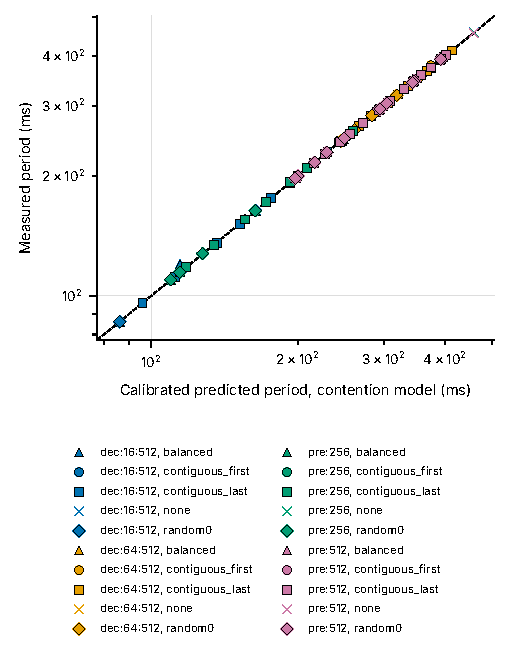
\includegraphics[width=0.75\linewidth]{figs/fig_accuracy.pdf}
\caption{Predicted versus measured iteration time for all streaming configurations of the main runs (Tesla T4, locked clocks). The line is $y=x$.}
\label{fig:accuracy}
\end{figure}

\subsection{Placement}
\label{sec:res-placement}

Figure~\ref{fig:penalty} shows, for each prefill length, the iteration time of the contiguous and balanced placements relative to the lower bound $\max(\sum c_i,\sum_{\text{streamed}} f_i)$ as the number of resident layers grows. The three regimes of Section~\ref{sec:theory} are visible. In the transfer-bound workloads ($T\le\nTransferBoundMaxT$, $f/c$ between \nRatioTransferMin{} and \nRatioTransferMax) the balanced placement stays at the bound for every $r$, while the contiguous one leaves the bound as soon as resident computation exceeds what $k$ slots can prefetch, and the gap widens until the resident layers' computation matches the streamed layers' copies. The largest measured gap is \nMeasPenaltyMax$\times$ (prefill of 256 tokens, $r=\nMeasPenaltyMaxR$, $k=\nMeasPenaltyMaxK$), and Theorem~\ref{thm:contig} predicts \nPredPenaltyAtMax$\times$. Contiguous-last behaves like contiguous-first, as the theory expects for any single block. Random placements fall in between; one random set of 21 layers that happened to contain a long resident run was \nRandomWorstPct\% slower than balanced. When a layer computes longer than it copies ($T\ge\nComputeBoundMinT$), all placements are within \nComputeBoundSpreadPct\% of each other and of the all-resident time, as Theorem~\ref{thm:compute} states. In decode the copies dominate unless almost all layers are resident, and placement matters only in the few configurations in which $rc$ approaches $mf$.

\begin{figure}[t]
\centering
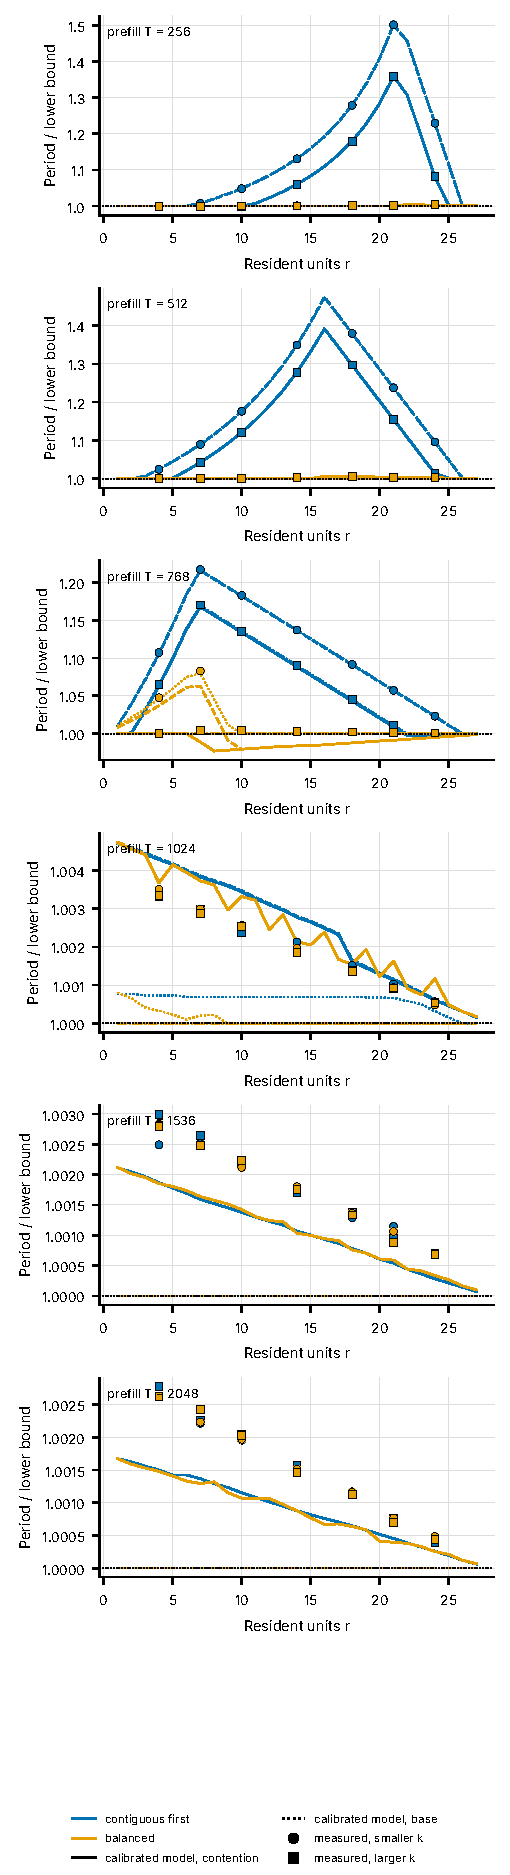
\includegraphics[width=\linewidth]{figs/fig_penalty.pdf}
\caption{Iteration time relative to the lower bound versus the number of resident layers, for contiguous-first and balanced placements (markers: measured; lines: model).}
\label{fig:penalty}
\end{figure}

Figure~\ref{fig:timeline} shows why. In the contiguous configuration the copy engine fills the slots while the resident block computes and then waits for most of the block; afterwards the streamed layers run at the copy rate. In the balanced configuration the copy engine is never idle and the iteration ends when the last copy has been consumed.

\begin{figure}[t]
\centering
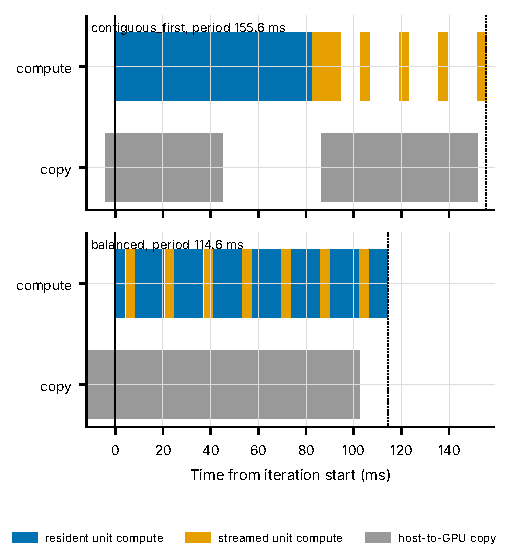
\includegraphics[width=\linewidth]{figs/fig_timeline.pdf}
\caption{Measured timelines of one iteration (prefill of 256 tokens, $r=21$, $k=3$) for contiguous-first (top) and balanced (bottom) placement. Each panel shows computation (upper row) and copies (lower row).}
\label{fig:timeline}
\end{figure}

\subsection{Number of slots}
\label{sec:res-slots}

At $T=768$ a layer copies in \nSweepRatio{} times its compute time, inside the band $c<f<2c$ of Proposition~\ref{prop:two}. Figure~\ref{fig:slots} shows the slot sweep for $r=14$. One slot serialises copy and computation. With two slots the balanced placement is \nSweepTwoOverThreePct\% slower than with three, as the proposition allows, and more slots do not help, as Theorem~\ref{thm:balanced} predicts. The model reproduces the sweep with a mean error of \nSweepMape\%.

\begin{figure}[t]
\centering
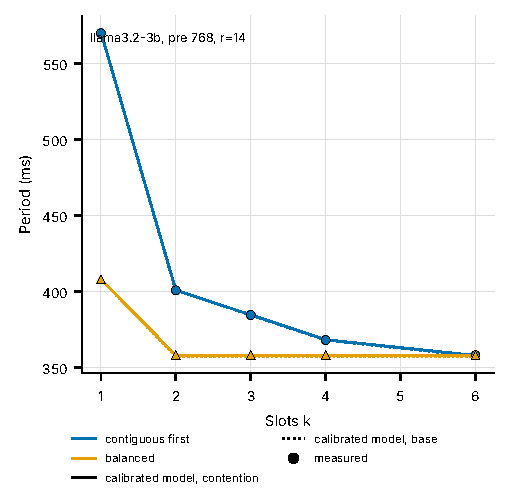
\includegraphics[width=0.75\linewidth]{figs/fig_slots.pdf}
\caption{Iteration time versus the number of slots at $T=768$, $r=14$ (markers: measured; lines: model).}
\label{fig:slots}
\end{figure}

\subsection{Non-uniform units: the output head}
\label{sec:res-nonuniform}

With the Llama-3.2 output head as an extra unit (788~MB, four times a layer, but computed for one token only), the model predicts the measured iterations with a mean error of \nHeadMape\%. Figure~\ref{fig:nonuniform} uses the measured per-unit times to compare placements under a memory budget. Streaming the head forces every slot to the head's size, so keeping the head resident and spreading the layers over the rest of the budget is \nNonUnifHeadGainPct\% faster than the balanced layer placement with a streamed head at the median budget; the local search finds placements within \nNonUnifLocalGainPct\% of this rule.

\begin{figure}[t]
\centering
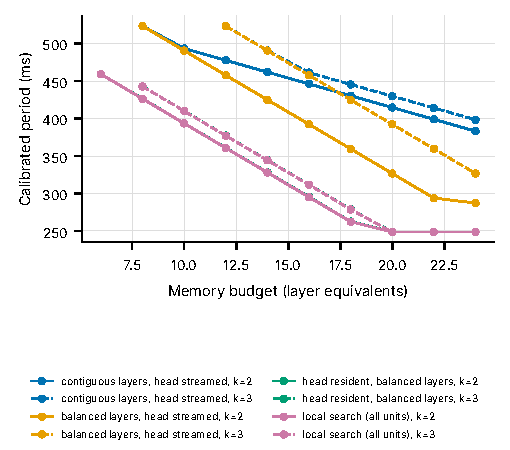
\includegraphics[width=0.75\linewidth]{figs/fig_nonuniform.pdf}
\caption{Predicted iteration time versus memory budget with the output head as a unit (prefill of 512 tokens): contiguous layers, balanced layers, head resident plus balanced layers, and local search.}
\label{fig:nonuniform}
\end{figure}

\subsection{Without clock locking}
\label{sec:res-power}

In runs whose SM clock fell below the locked value because of the power cap, the model with compute times from a cooler phase errs by up to \nCapMax\% (mean \nCapMape\%). Scaling each configuration's compute times by the ratio of the clock during the compute measurement to the clock during the run removes almost all of it (mean \nCapClockMape\%, maximum \nCapClockMax\%), so the error is the clock, not the pipeline model. In our first, fully unlocked runs the effect changed a conclusion: for a 1\,024-token prefill with 14 resident layers the balanced placement measured 374~ms against 364~ms for the contiguous one, although the model predicts the opposite. These runs had no clock samples, so we can only point to the mechanism shown above: with a balanced placement copies overlap computation for the whole iteration, which raises power draw and lowers the clock exactly while the computation is on the critical path.


%% ===================================================================
\section{Discussion}
\label{sec:discussion}

\paragraph{What runtimes should do}
The rules of Section~\ref{sec:theory} cost nothing to apply. A runtime that streams layers with prefetching should spread its resident layers evenly instead of filling GPU memory in model order, and should size its ring by the ratio of copy to compute time per layer: two slots when a copy takes at least twice as long as a layer's computation, three otherwise, or the faster of the two according to the evaluator, which needs only per-layer compute and copy times that a runtime can measure in one iteration. When a layer computes longer than it takes to copy, resident layers do not shorten the iteration at all, and the memory is better spent on a larger batch or key--value cache. When copies dominate even with every free byte resident, placement does not matter either, and only fewer bytes (quantisation) or a faster path help.

\paragraph{Faster paths and CXL memory}
The analysis depends on the path only through the copy time per layer $f$. A CXL Type-3 expander reached through a page-locked host mapping is such a path \cite{yoon2025tract,jang2026itme}, and reported bandwidths for current devices are of the order we measured on PCIe Gen3. If copies from such a device take a constant time per layer, the theorems apply to it as stated. Whether they do is an open question that our measurements cannot answer: copies from an unpinned CXL region go through a bounce buffer \cite{yoon2025tract}, and contention on a shared device or with host memory traffic would make $f$ vary from copy to copy. A faster path, such as several expanders interleaved or PCIe Gen5, lowers $f$ and moves a given workload towards the regime $f\le c$ in which placement no longer matters; a GPU that computes faster moves it the other way.

\paragraph{Power-limited GPUs}
On the power-limited T4 a concurrent copy and long runs lowered the SM clock, which changes $c$ during an iteration and breaks assumption A4. The effect was large enough to reverse the order of two placements in one configuration of our first runs (Section~\ref{sec:res-power}). The contention variant of the model captures the part caused by concurrent copies but not the slower drift of the clock with temperature and power. Data-centre GPUs with higher power limits are less affected, but any deployment that runs close to its power limit should measure $c$ under the same conditions as the iteration it wants to predict.

\paragraph{Limitations}
(i) All measurements are on one GPU type, a power-limited T4 on Colab virtual machines, with two model shapes. The clock lock that makes the measurements reproducible runs the GPU at about a third of its maximum clock, which shifts every workload towards larger $f/c$; on a faster GPU or at default clocks the same workload has a smaller $c$ and the regime boundaries move. (ii) The layer kernels omit rotary embeddings, expand grouped key--value heads explicitly, and share one read-only key--value cache across layers; each configuration is measured once, with one random placement per cell. (iii) The runtime is written in Python without CUDA graphs, and in the shortest decode iterations host launch overhead, which the model ignores, may be on the critical path. (iv) We stream whole layers; a runtime that splits layers into tensors has more, smaller units, to which Lemma~\ref{lem:cycle} applies unchanged but for which we did not measure. (v) The key--value cache stays in GPU memory; streaming it as well adds per-layer copy time that grows with the context, which fits the model as a larger $f_i$ but was not measured. (vi) We assume one copy engine and in-order execution; runtimes that reorder layers or split copies across several engines need a different event graph. (vii) The theorems cover layers of equal cost and require $k\le m$; for non-uniform units we offer an exact evaluator and a search, not a closed form.


%% ===================================================================
\section{Conclusion}
\label{sec:conclusion}

Streaming the layers of a model through a small GPU-memory ring is a max-plus linear system, and its iteration time is the maximum mean of a family of tilings of the layer sequence. For layers of equal cost this gives a complete answer to the placement question. When a layer computes at least as long as its copy takes, two slots suffice and resident layers are useless. Otherwise, spreading the resident layers evenly attains the lower bound $\max(Lc,mf)$ as soon as $(k-1)f\ge2c$, while a contiguous block, the result of filling GPU memory in model order, takes $\max(Lc,mf,rc+2c+(m-k)f)$, up to twice as long. On a Tesla T4 with page-locked host memory, the same bandwidth class as current CXL expanders, the model predicted \nAccN{} measured iteration times with a mean error of \nAccMape\%, and even spreading was up to \nMeasPenaltyMax$\times$ faster than the contiguous prefix. The rules are cheap enough for any offloading runtime to adopt; the open questions are tensor-level units, streamed key--value caches and power-limited operation, in which the per-layer times themselves depend on the schedule.


\section*{CRediT authorship contribution statement}
\textbf{Quang-Vinh Dang}: Conceptualization, Methodology, Formal analysis, Software, Investigation, Writing -- original draft, Visualization, Supervision. \textbf{Dat Le}: Validation, Writing -- review \& editing. \textbf{Minh Ngoc Dinh}: Validation, Writing -- review \& editing.

\section*{Data availability}
The model code, the GPU runtime, the raw measurements and the scripts that produce every number, table and figure are available at \url{https://github.com/vinhqdang/Enabling-CXL-Based-Memory-Disaggregation-for-Large-Scale-AI-Systems}.

\section*{Funding}
This research did not receive any specific grant from funding agencies in the public, commercial, or not-for-profit sectors.

\section*{Declaration of competing interest}
The authors declare that they have no known competing financial interests or personal relationships that could have appeared to influence the work reported in this paper.

\section*{Declaration of generative AI and AI-assisted technologies in the manuscript preparation process}
During the preparation of this work the authors used generative AI-assisted tools for software implementation, experiment scripting and drafting and editing of text. After using these tools, the authors reviewed, verified and edited all code, results and content as needed and take full responsibility for the content of the published article.

\bibliographystyle{elsarticle-num}
\bibliography{refs}

\end{document}
